\chapter{Menginputkan File Excel Ke Dalam Database APEX}

\begin{enumerate}
\item[1]Buat Data mahasiswa di excel dengan format .xlsx.
\item[2]Masuk ke dalam Oracle APEX online Dan buat Workspace baru.
\item[3]Isikan data diri anda seperti nama,email,dan nama workspace yang akan dibuat dan jangan sampai lupa.
\item[4]Centang apakah anda pernah melakukan hal yang tanyakan dibawah lalu next. \begin{figure}[!htbp]
    \begin{center}
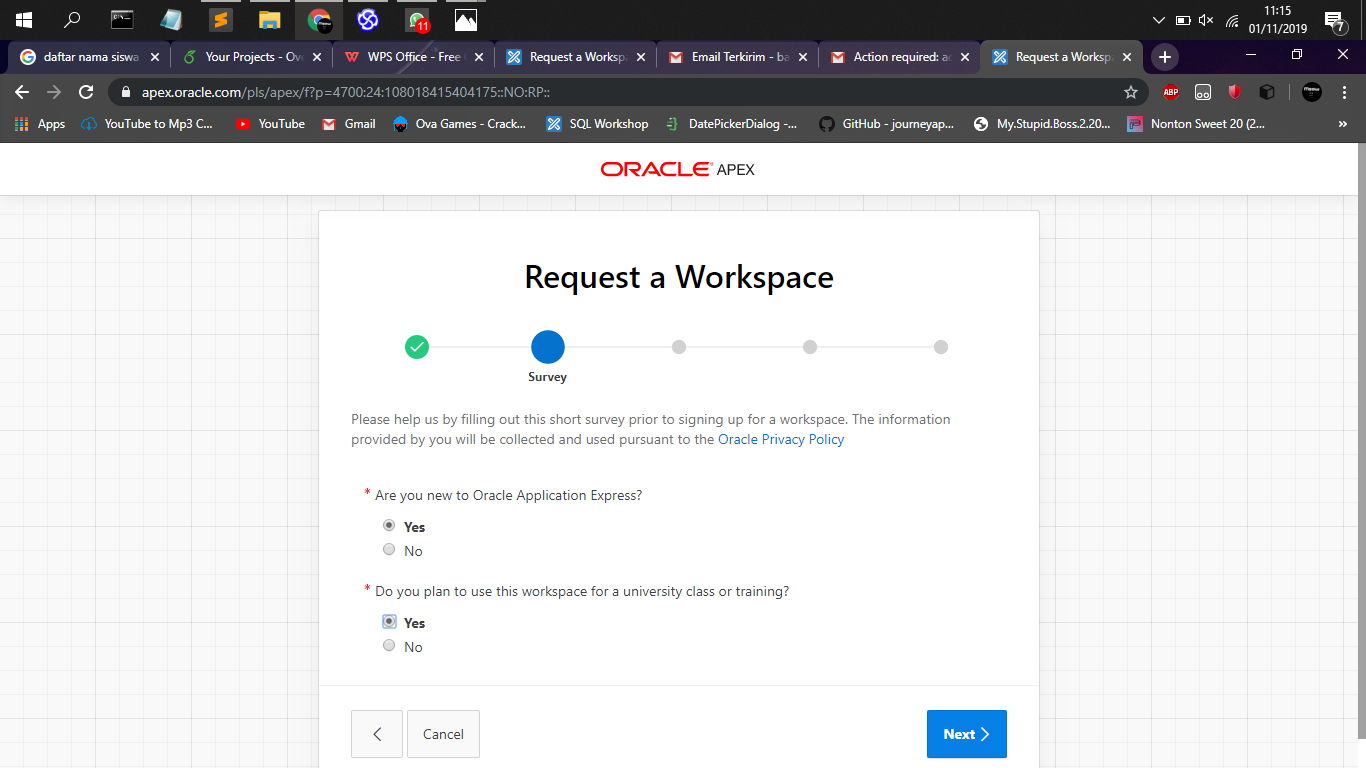
\includegraphics[scale=0.2]{figures/3.png}
    \caption{\textit{Data Diri 2.}}
        \end{center}
        \end{figure}
\begin{figure}
\item[5]Isikan alasan mengapa anda ingin menggunakan layanan ini ?, lalu klik next.

    \begin{center}
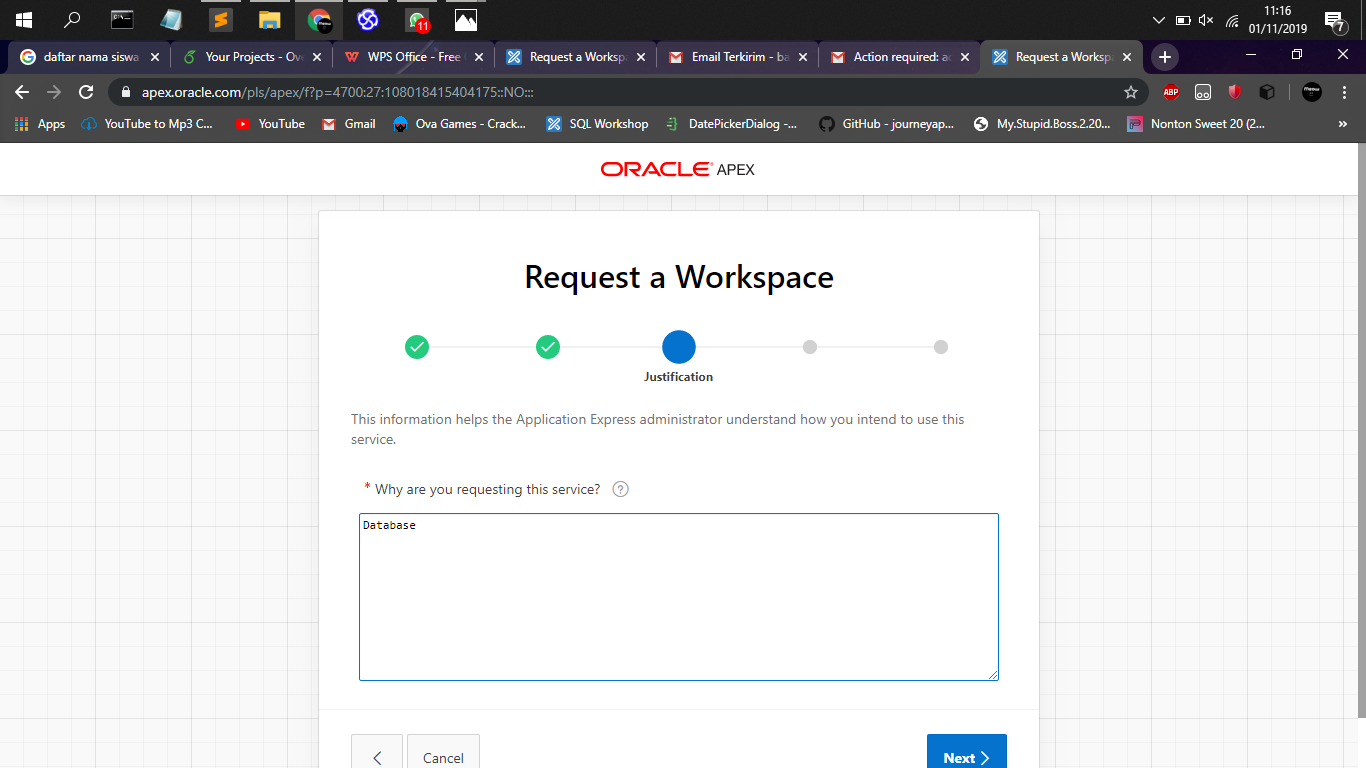
\includegraphics[scale=0.2]{figures/4.png}
    \caption{\textit{Mengapa anda menggunakan oracle ?.}}
        \end{center}

\label{gambar}
\end{figure}

\begin{figure}
\item[6] Centang Accept, lalu klik next.

    \begin{center}
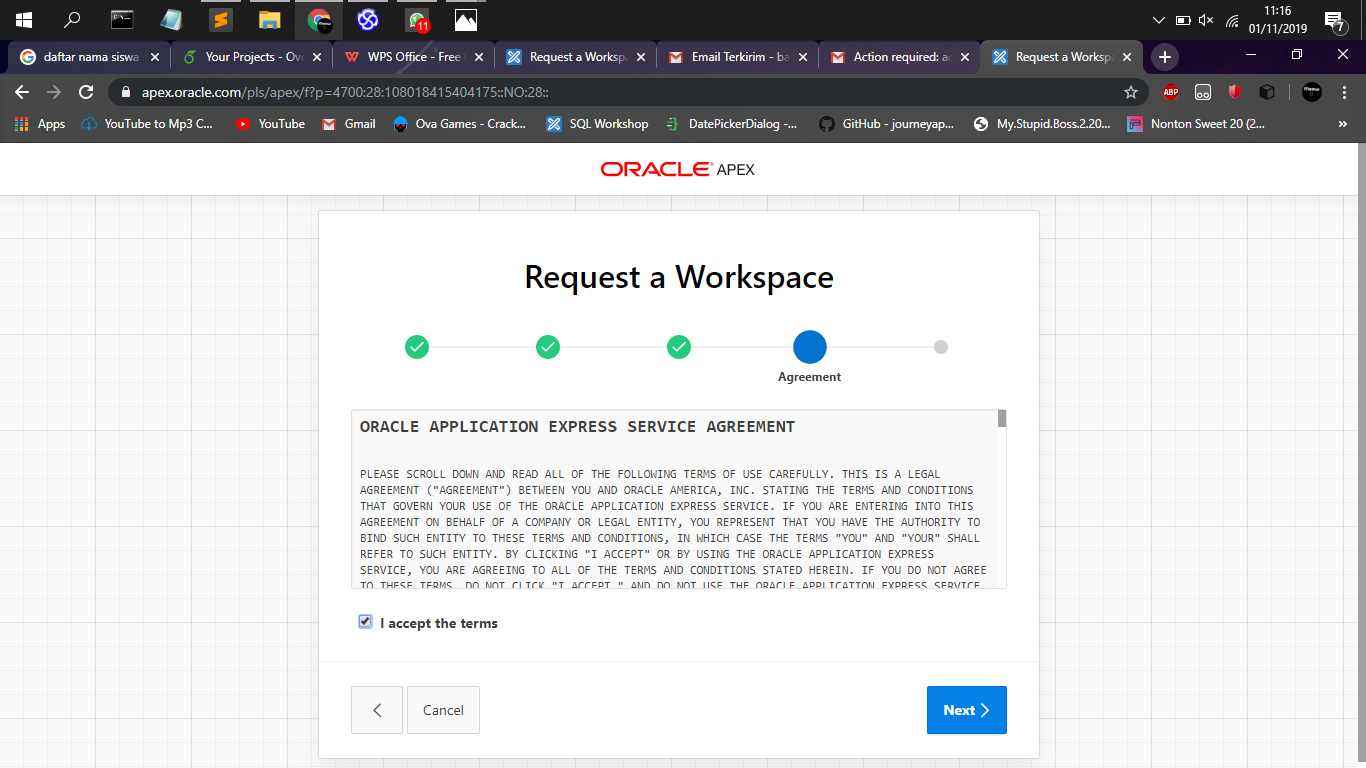
\includegraphics[scale=0.2]{figures/5.png}
    \caption{\textit{Peringatan pengunaan.}}
        \end{center}

\label{gambar}
\end{figure}

\begin{figure}
\item[7] Tahapan terakhir untuk mengkonfirmasi apakah ini anda, lalu klik next.

    \begin{center}
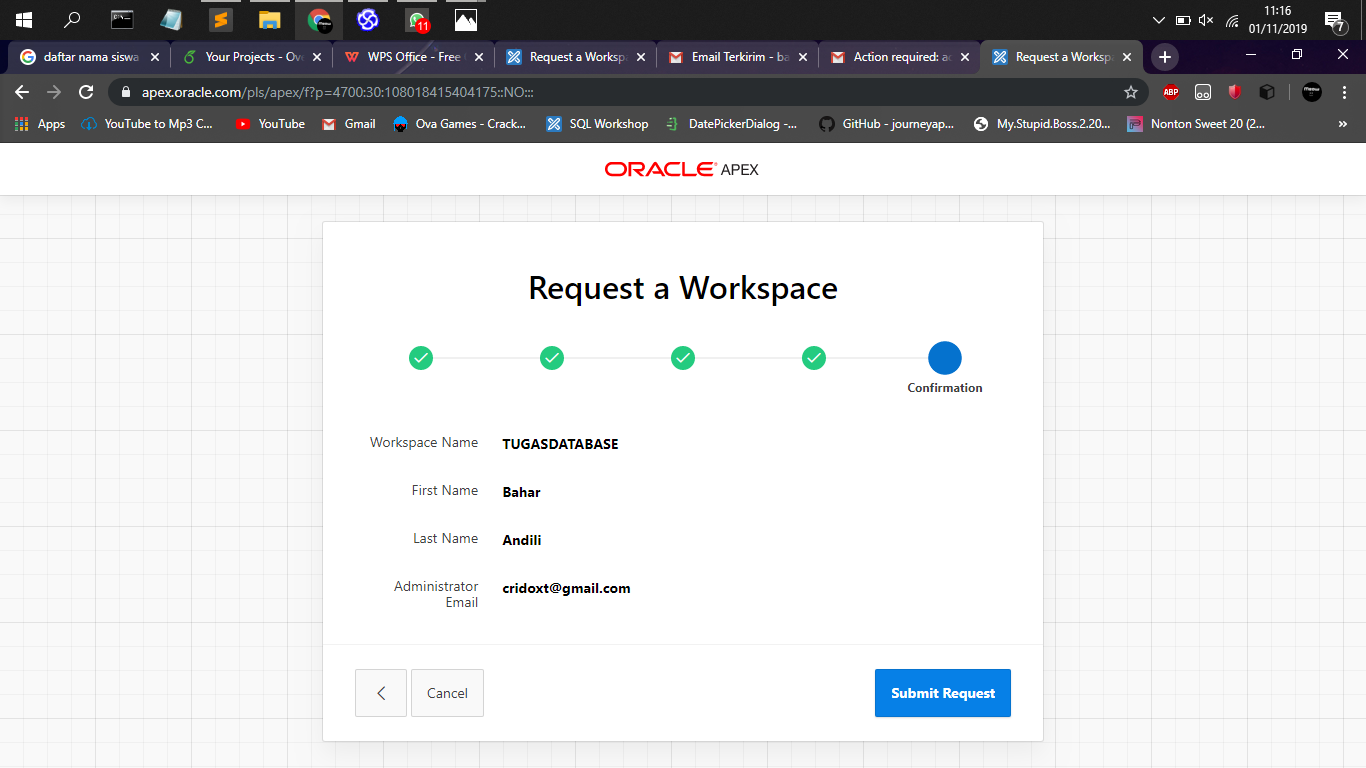
\includegraphics[scale=0.2]{figures/6.png}
    \caption{\textit{Konfirmasi.}}
        \end{center}
\label{gambar}
\end{figure}

\begin{figure}
\item[8] Finish, lalu lihat email anda.

    \begin{center}
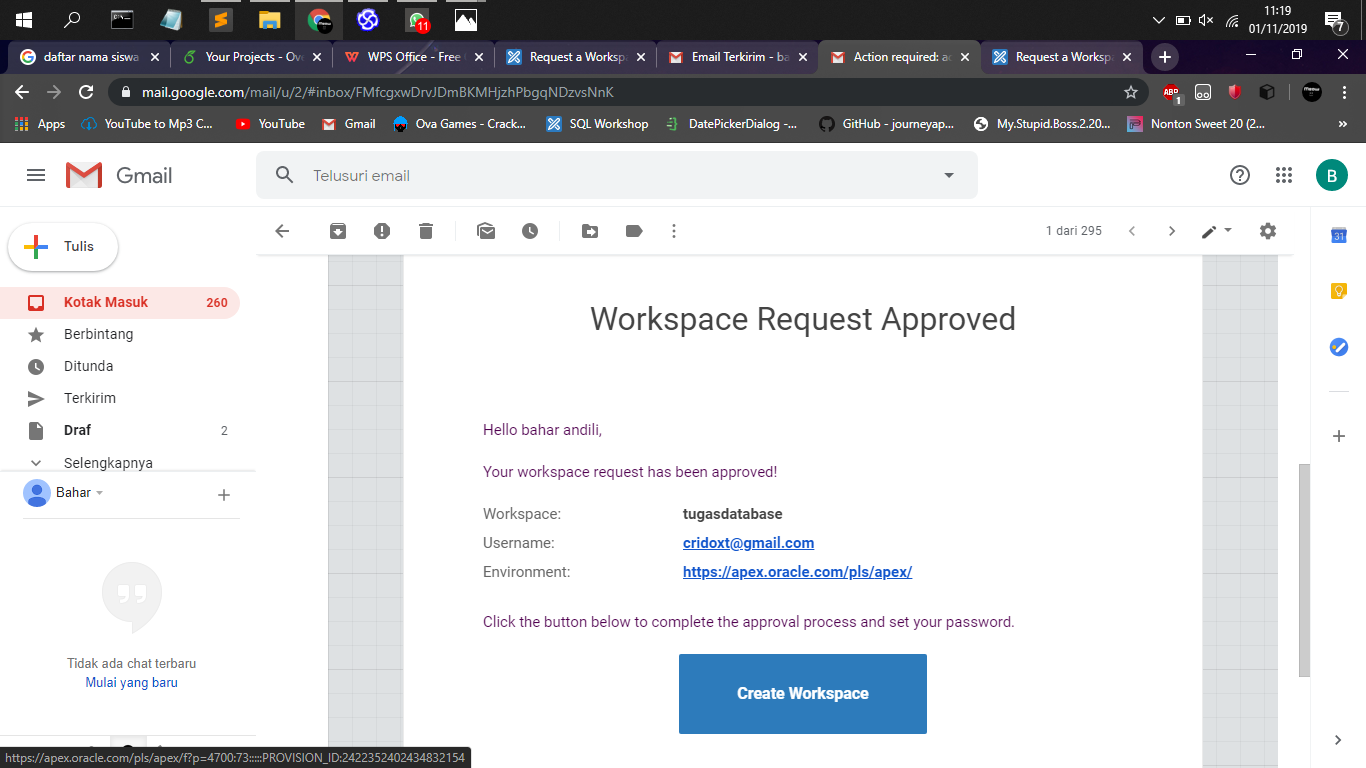
\includegraphics[scale=0.2]{figures/7.png}
    \caption{\textit{Sukses Cek Email.}}
        \end{center}
\label{gambar}
\end{figure}

\begin{figure}
\item[9] Selamat Workspace anda telah di Acc lalu klik continue.

    \begin{center}
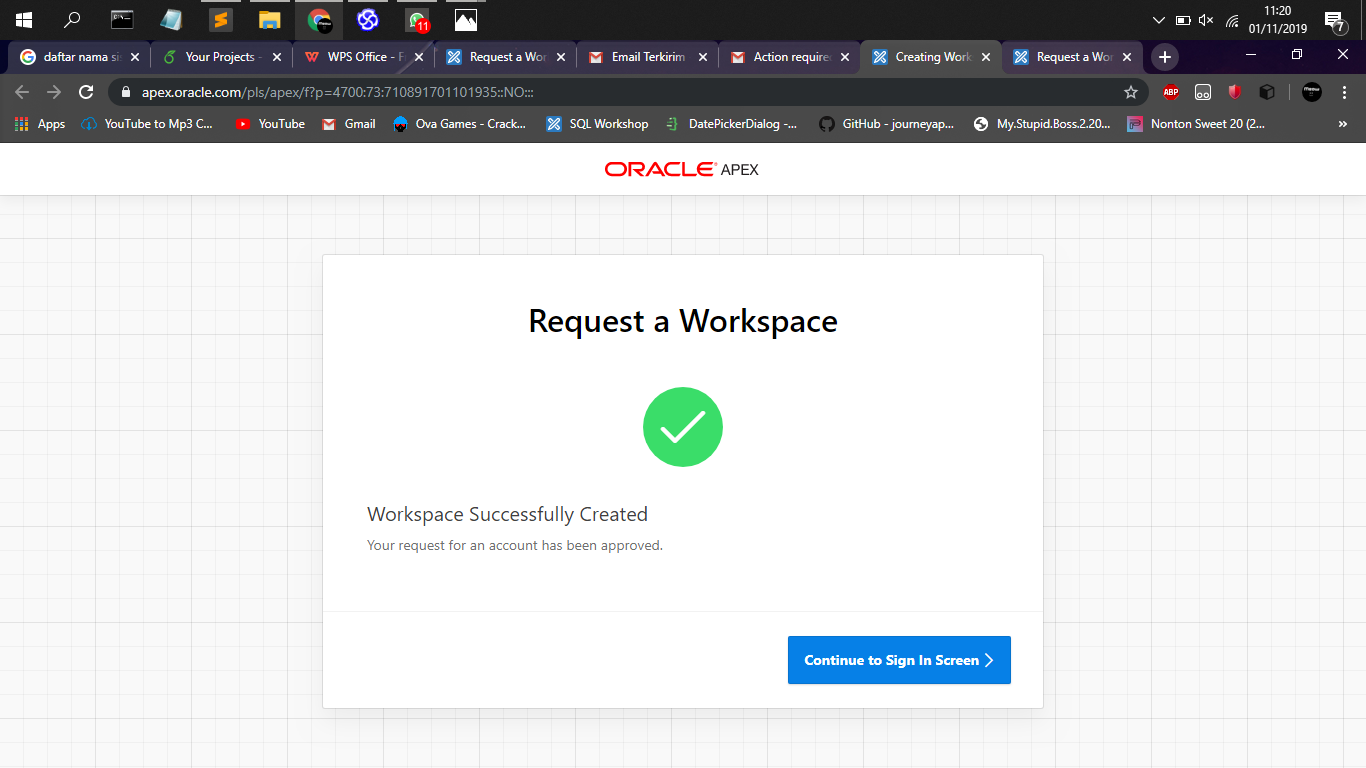
\includegraphics[scale=0.2]{figures/8.png}
    \caption{\textit{Email Acc.}}
        \end{center}
\label{gambar}
\end{figure}

\begin{figure}
\item[10] Workspace kamu telah dibut lalu lanjutkan dengan sign in.
\label{gambar}
\end{figure}

\begin{figure}
\item[11] Masuk kedalam menu database oracle APEX dan klik App Bulider .
\label{gambar}
\end{figure}
\begin{figure}
\item[12] Klik create.
\label{gambar}
\end{figure}
\begin{figure}
\item[13]setelah Create New App pilih From A File dari file.
\label{gambar}
\end{figure}

\begin{figure}
\item[14] Pilih File yang akan di inputkan ke dalam aplikasi.
\label{gambar}
\end{figure}

\begin{figure}
\item[15] Scroll ke bwah lalu setting Table Owner,Table Name,Error Table Name, dan Primary Keys.
\label{gambar}
\end{figure}

\begin{figure}
\item[16] Load data.
\label{gambar}
\end{figure}

\begin{figure}
\item[17] Kemudian, scroll kebawah dan Check All dan Create Application. 
\label{gambar}
\end{figure}

\begin{figure}
\item[18] Kemudian Run Application.
\label{gambar}
\end{figure}

\begin{figure}
\item[19]Masukkan username dan password workspace tadi.

ferdyberliano8@gmail.com


08032001


https://apex.oracle.com/pls/apex/f?p=34628:3:15522284854553::NO:::
\label{gambar}
\end{figure}

\begin{figure}
\item[20]Tampilan Aplication .
\label{gambar}
\end{figure}

\begin{figure}
\item[21]Tabel data.
    \begin{center}
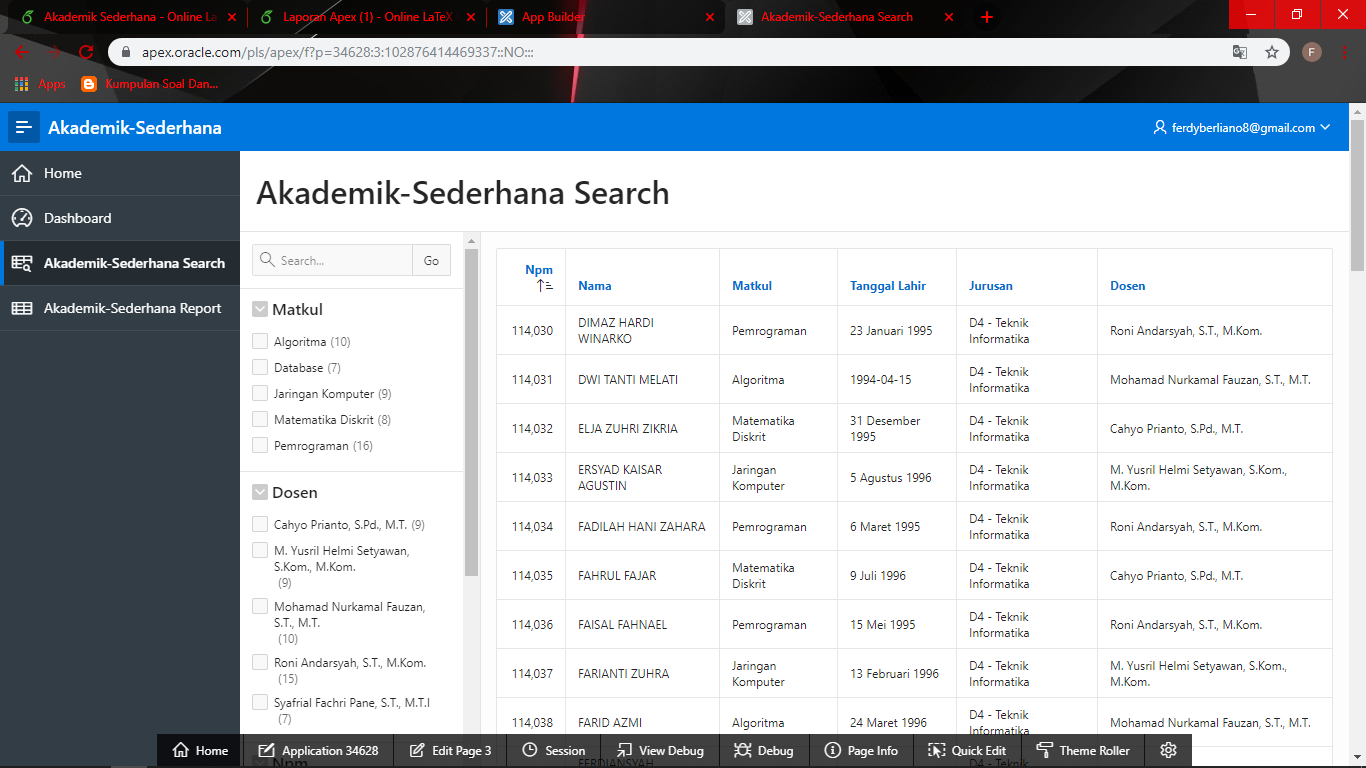
\includegraphics[scale=0.2]{figures/20.png} 
    \caption{\textit{Tampilan data mahasiswa.}}
        \end{center}
\label{gambar}
\end{figure}
\end{enumerate}

